\documentclass[11pt,a4paper]{article}

\usepackage[utf8]{inputenc}
\usepackage[T1]{fontenc}
\usepackage{lmodern}
\usepackage{float}
\usepackage[margin=2cm]{geometry}
\usepackage{amsmath,amssymb}
\usepackage{booktabs}
\usepackage{graphicx}
\usepackage{hyperref}
\usepackage{xcolor}
\usepackage{titlesec}
\usepackage{tabularx}
\usepackage{subcaption}

\hypersetup{
    colorlinks=true,
    linkcolor=blue!70!black,
    citecolor=blue!70!black,
    urlcolor=blue!70!black
}

\titleformat{\section}
{\large\bfseries}{\thesection.}{0.5em}{}
\titleformat{\subsection}
{\normalsize\bfseries}{\thesubsection.}{0.5em}{}
\titlespacing*{\section}{0pt}{1.2ex plus 0.5ex minus .2ex}{0.6ex}
\titlespacing*{\subsection}{0pt}{1.0ex plus 0.4ex minus .2ex}{0.4ex}

\setlength{\parskip}{0.45em}
\setlength{\parindent}{0pt}

\begin{document}

\begin{center}
{\LARGE \textbf{Projeto 3: Modelo Generativo (VAE) para Fashion-MNIST}} \\[0.35em]
{\large Disciplina: Introdução às Redes Neurais Artificiais} \\[0.3em]
\textbf{Autor:} Gabriely Di Folco Rocha \\[0.2em]
\textbf{Repositório:} \url{https://github.com/ghostfoxgoddes3/ANN}
\end{center}

\vspace{-0.5em}
\hrule
\vspace{0.8em}

\section{Objetivo e Escopo}

Este projeto treina um modelo generativo do tipo \textit{Variational
Autoencoder} (VAE) sobre o conjunto Fashion-MNIST. O objetivo é duplo: (i)
ajustar a topologia do modelo de modo a minimizar a função de custo no conjunto
de validação, considerando duas configurações de espaço latente, com 2 e 8
dimensões; e (ii) explorar o espaço latente aprendido, verificando a formação
de \textit{clusters}, a separação dos rótulos e, no caso 8D, quanto da variância
uma projeção bidimensional consegue ilustrar.

O Fashion-MNIST contém imagens em tons de cinza de $28\times28$ pixels,
distribuídas em dez classes de vestuário: \textit{T-shirt/top}, \textit{Trouser},
\textit{Pullover}, \textit{Dress}, \textit{Coat}, \textit{Sandal},
\textit{Shirt}, \textit{Sneaker}, \textit{Bag} e \textit{Ankle boot}. Cada
imagem é tratada como um vetor $\mathbf{x}\in[0,1]^{784}$, obtido dividindo-se
os valores de pixel por 255.

\section{Formulação do VAE}

O VAE é um modelo latente que assume um gerador
$p_\theta(\mathbf{x}\mid\mathbf{z})$ e um \textit{prior} $p(\mathbf{z})=
\mathcal{N}(\mathbf{0},\mathbf{I})$. Como a posterior verdadeira é intratável,
introduz-se um codificador $q_\phi(\mathbf{z}\mid\mathbf{x})$ e otimiza-se o
limite inferior da evidência (ELBO). A função de custo minimizada é o ELBO
negativo:
\[
\mathcal{L}(\mathbf{x})=
\underbrace{\mathbb{E}_{q_\phi(\mathbf{z}\mid\mathbf{x})}
\!\left[-\log p_\theta(\mathbf{x}\mid\mathbf{z})\right]}_{\text{reconstrução}}
\;+\;
\beta\,
\underbrace{D_{\mathrm{KL}}\!\left(q_\phi(\mathbf{z}\mid\mathbf{x})\,\|\,
p(\mathbf{z})\right)}_{\text{regularização}} .
\]
O termo de reconstrução foi implementado como entropia cruzada binária entre a
imagem original e a reconstruída, somada sobre os 784 pixels e promediada por
amostra. O termo KL possui forma fechada para posteriors gaussianas
diagonais:
\[
D_{\mathrm{KL}}=-\tfrac{1}{2}\sum_{j=1}^{d}
\left(1+\log\sigma_j^2-\mu_j^2-\sigma_j^2\right),
\]
em que $d$ é a dimensão latente. Utilizou-se $\beta=1$ (VAE padrão). A
amostragem de $\mathbf{z}$ emprega o truque de reparametrização,
$\mathbf{z}=\boldsymbol{\mu}+\boldsymbol{\sigma}\odot\boldsymbol{\epsilon}$,
com $\boldsymbol{\epsilon}\sim\mathcal{N}(\mathbf{0},\mathbf{I})$, o que permite
a retropropagação através da operação estocástica.

Tanto o codificador quanto o decodificador são MLPs com ativação ReLU. O
codificador termina em duas camadas lineares paralelas, para $\boldsymbol{\mu}$
e $\log\boldsymbol{\sigma}^2$; o decodificador reflete a topologia do
codificador e termina em uma sigmoide, de modo que as saídas fiquem em $[0,1]$.

\section{Configuração Experimental e Reprodutibilidade}

\subsection{Partição dos dados}

O conjunto de treino original (60\,000 imagens) foi dividido em 54\,000 para
treino e 6\,000 para validação, com semente fixa igual a 42. O conjunto de
teste oficial, com 10\,000 imagens, foi mantido separado e utilizado apenas na
avaliação final e nas visualizações do espaço latente. A seleção de topologia
baseou-se exclusivamente na loss de validação.

\subsection{Busca de topologia}

Para cada dimensão latente, foram comparadas três topologias de camadas
ocultas: $(256)$, $(512,256)$ e $(512,256,128)$. A mesma topologia é usada no
codificador e, de forma espelhada, no decodificador. O otimizador foi o Adam
com taxa de aprendizado $10^{-3}$ e tamanho de lote 256. Para acelerar a busca
em ambiente apenas com CPU, cada candidato foi treinado por até 8 épocas sobre
uma subamostra de 20\,000 imagens de treino, com parada antecipada
(\textit{patience} 3) monitorando a loss de validação. A configuração de menor
loss de validação foi então re-treinada por até 20 épocas sobre o conjunto de
treino completo (54\,000 imagens), com \textit{patience} 6.

\begin{table}[H]
\centering
\small
\caption{Espaço de busca e condições comuns a todos os experimentos.}
\label{tab:setup}
\begin{tabularx}{\textwidth}{lX}
\toprule
\textbf{Item} & \textbf{Valor} \\
\midrule
Dimensões latentes & 2 e 8 \\
Topologias ocultas & $(256)$, $(512,256)$, $(512,256,128)$ \\
Ativação & ReLU (saída do decodificador: sigmoide) \\
Otimizador & Adam, $\eta=10^{-3}$ \\
Tamanho de lote & 256 \\
Peso KL & $\beta = 1$ \\
Reconstrução & Entropia cruzada binária (soma por imagem) \\
Épocas (busca / final) & 8 / 20, com parada antecipada \\
Subamostra na busca & 20\,000 imagens \\
Semente & 42 \\
\bottomrule
\end{tabularx}
\end{table}

\section{Resultados da Otimização}

\subsection{Seleção da topologia}

A Tabela~\ref{tab:search} resume a busca. Para o espaço latente 2D, a loss de
validação diminuiu monotonicamente com a profundidade da rede, e a topologia
$(512,256,128)$ foi selecionada. Para o espaço 8D, a topologia intermediária
$(512,256)$ apresentou a menor loss de validação, superando tanto a rede rasa
quanto a mais profunda dentro do orçamento de treino utilizado.

\begin{table}[H]
\centering
\small
\caption{Busca de topologia. Loss de validação (ELBO negativo) por candidato.}
\label{tab:search}
\begin{tabular}{llrr}
\toprule
\textbf{Latente} & \textbf{Topologia} & \textbf{Parâmetros} & \textbf{Loss val.} \\
\midrule
2D & $(256)$          & 404\,244    & 277,351 \\
2D & $(512,256)$      & 1\,068\,820 & 266,938 \\
2D & $(512,256,128)$  & 1\,133\,844 & \textbf{264,868} \\
\midrule
8D & $(256)$          & 408\,864    & 254,109 \\
8D & $(512,256)$      & 1\,073\,440 & \textbf{248,586} \\
8D & $(512,256,128)$  & 1\,136\,160 & 252,269 \\
\bottomrule
\end{tabular}
\end{table}

\subsection{Modelos finais}

A Tabela~\ref{tab:final} apresenta o desempenho dos modelos re-treinados. Em
ambos os espaços, o teste reproduz de perto a validação, sem sinais de
sobreajuste severo. O modelo 8D alcança reconstrução nitidamente melhor
(227,9 contra 251,5 no teste), ao custo de um termo KL maior (12,7 contra 6,7):
dimensões latentes adicionais carregam mais informação sobre cada imagem e, por
isso, afastam-se mais do \textit{prior}.

\begin{table}[H]
\centering
\small
\caption{Desempenho final dos VAEs selecionados. Valores por imagem.}
\label{tab:final}
\begin{tabular}{llrrrr}
\toprule
\textbf{Latente} & \textbf{Topologia} & \textbf{Loss val.} &
\textbf{Loss teste} & \textbf{Recon. teste} & \textbf{KL teste} \\
\midrule
2D & $(512,256,128)$ & 255,623 & 258,167 & 251,497 & 6,671 \\
8D & $(512,256)$     & 238,254 & 240,676 & 227,942 & 12,734 \\
\bottomrule
\end{tabular}
\end{table}

As curvas de treino (Figuras~\ref{fig:hist2d} e~\ref{fig:hist8d}) decompõem a
loss de validação em reconstrução e KL ao longo das épocas. Em ambos os casos,
a reconstrução é o componente dominante da loss, e o termo KL estabiliza em um
patamar coerente com a dimensão latente.

\begin{figure}[H]
\centering
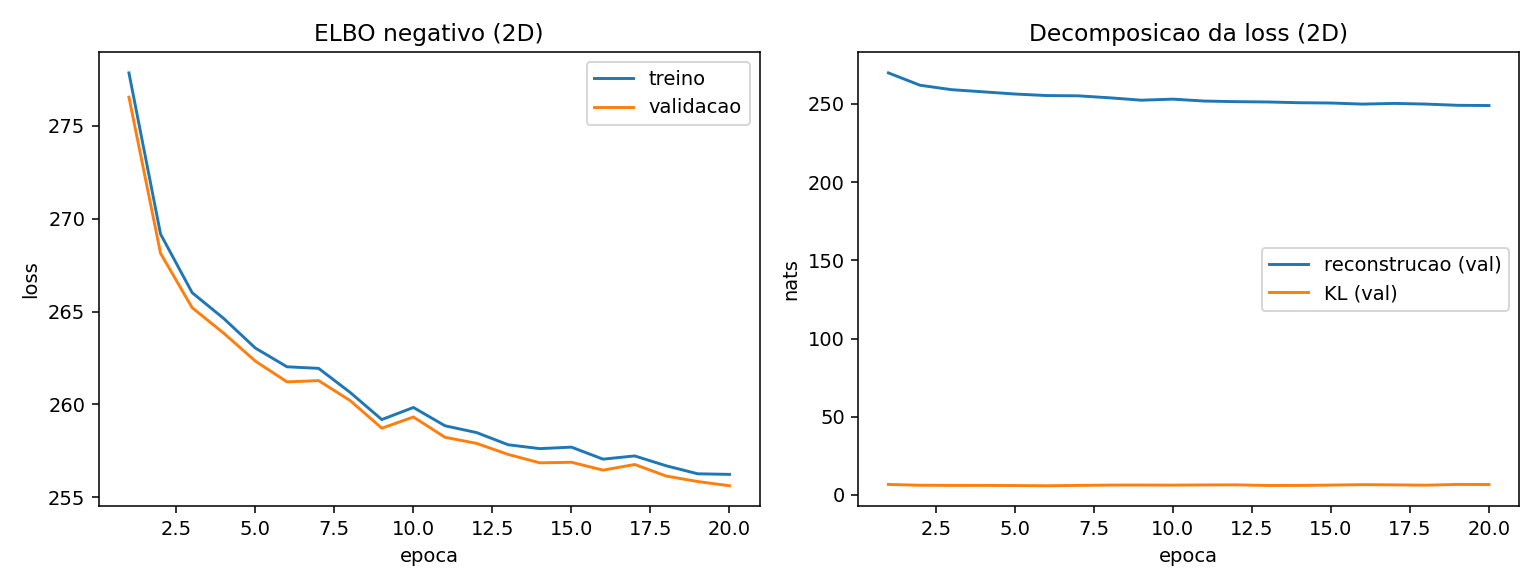
\includegraphics[width=\textwidth]{../figures/history_latent2.png}
\caption{Dinâmica de treino do VAE 2D: ELBO negativo (esquerda) e decomposição
da loss de validação em reconstrução e KL (direita).}
\label{fig:hist2d}
\end{figure}

\begin{figure}[H]
\centering
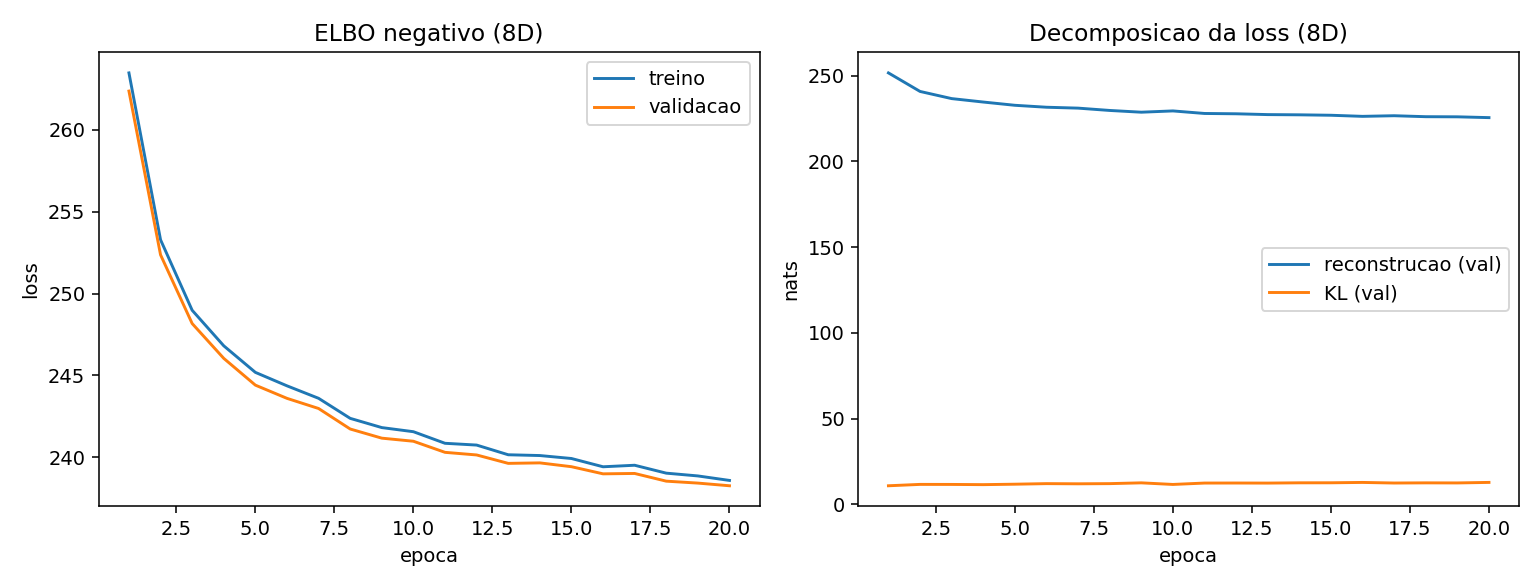
\includegraphics[width=\textwidth]{../figures/history_latent8.png}
\caption{Dinâmica de treino do VAE 8D: ELBO negativo (esquerda) e decomposição
da loss de validação em reconstrução e KL (direita).}
\label{fig:hist8d}
\end{figure}

\subsection{Qualidade da reconstrução}

As Figuras~\ref{fig:rec2d} e~\ref{fig:rec8d} comparam imagens originais e suas
reconstruções. O VAE 2D captura a silhueta geral das peças, mas perde textura e
detalhes finos, efeito esperado de um gargalo de apenas duas dimensões. O VAE
8D produz reconstruções visivelmente mais nítidas, consistentes com o menor erro
de reconstrução da Tabela~\ref{tab:final}.

\begin{figure}[H]
\centering
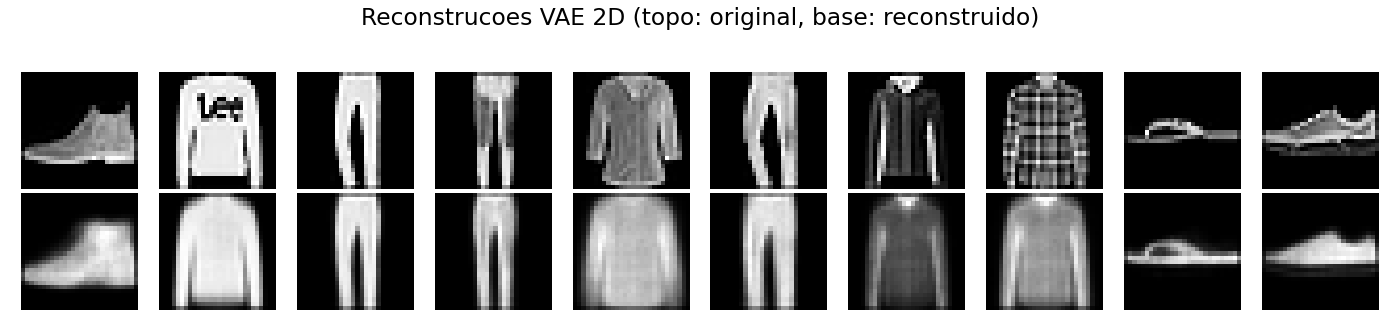
\includegraphics[width=0.9\textwidth]{../figures/reconstructions_latent2.png}
\caption{Reconstruções do VAE 2D (linha superior: original; inferior:
reconstruída).}
\label{fig:rec2d}
\end{figure}

\begin{figure}[H]
\centering
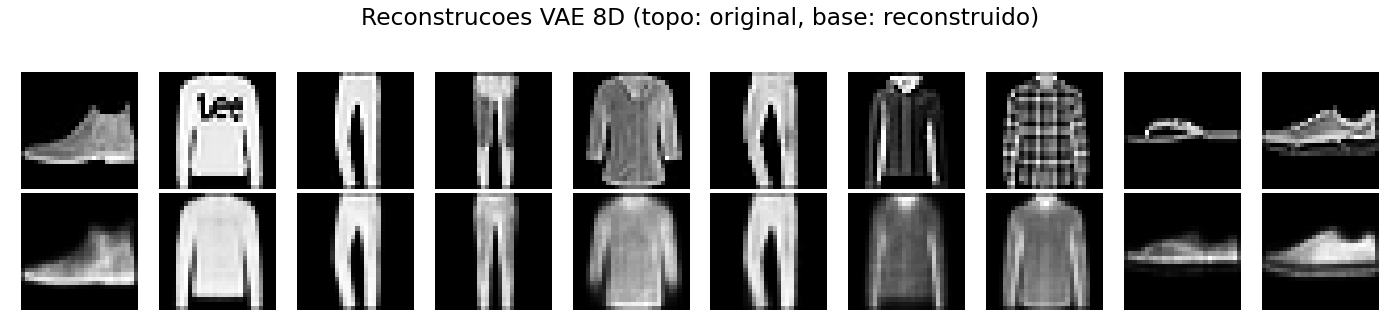
\includegraphics[width=0.9\textwidth]{../figures/reconstructions_latent8.png}
\caption{Reconstruções do VAE 8D (linha superior: original; inferior:
reconstruída).}
\label{fig:rec8d}
\end{figure}

\section{Exploração do Espaço Latente}

Para explorar o espaço latente, codificou-se todo o conjunto de teste
(10\,000 imagens) usando a média $\boldsymbol{\mu}$ do posterior de cada
imagem. No caso 2D, as coordenadas são plotadas diretamente; no caso 8D,
aplicou-se PCA e projetaram-se os dois primeiros componentes principais. Os
pontos são coloridos pelos rótulos verdadeiros, que não participaram do treino
(o VAE é não supervisionado).

\subsection{Espaço latente 2D}

\begin{figure}[H]
\centering
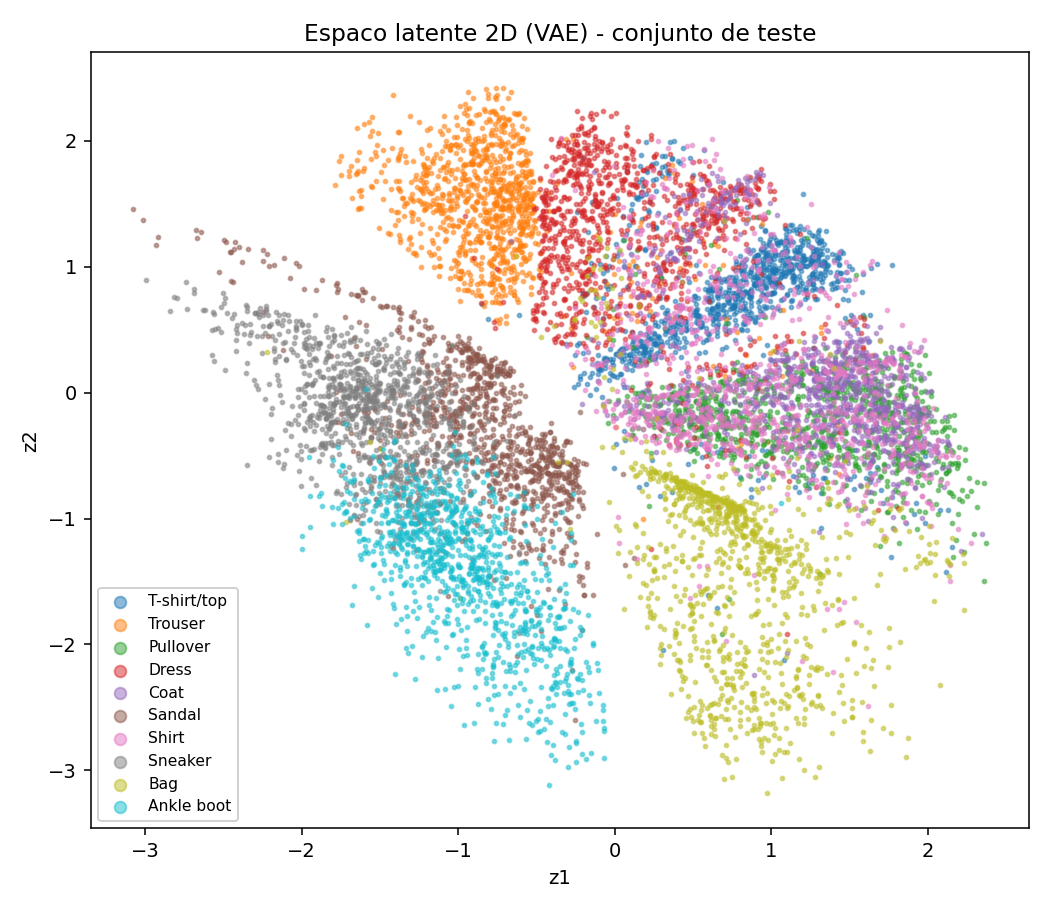
\includegraphics[width=0.74\textwidth]{../figures/latent2d_scatter.png}
\caption{Espaço latente 2D do VAE, colorido pelos rótulos do conjunto de teste.}
\label{fig:lat2d}
\end{figure}

A Figura~\ref{fig:lat2d} mostra organização clara. Os calçados ocupam a
metade esquerda e inferior do plano: \textit{Sneaker}, \textit{Sandal} e
\textit{Ankle boot} formam regiões contíguas, separadas do restante. A classe
\textit{Trouser} ocupa um aglomerado isolado no topo, e \textit{Bag} ocupa a
região inferior direita, também bem delimitada. Já as peças de parte superior do
corpo --- \textit{T-shirt/top}, \textit{Pullover}, \textit{Dress},
\textit{Coat} e \textit{Shirt} --- concentram-se à direita e apresentam forte
sobreposição entre si, o que é coerente com sua semelhança visual.

A Figura~\ref{fig:sweep2d} complementa a análise decodificando uma grade regular
de pontos do plano latente. A transição suave entre tipos de peça ao percorrer o
plano indica que o espaço aprendido é contínuo e organizado por similaridade de
forma, propriedade característica de um bom modelo generativo.

\begin{figure}[H]
\centering
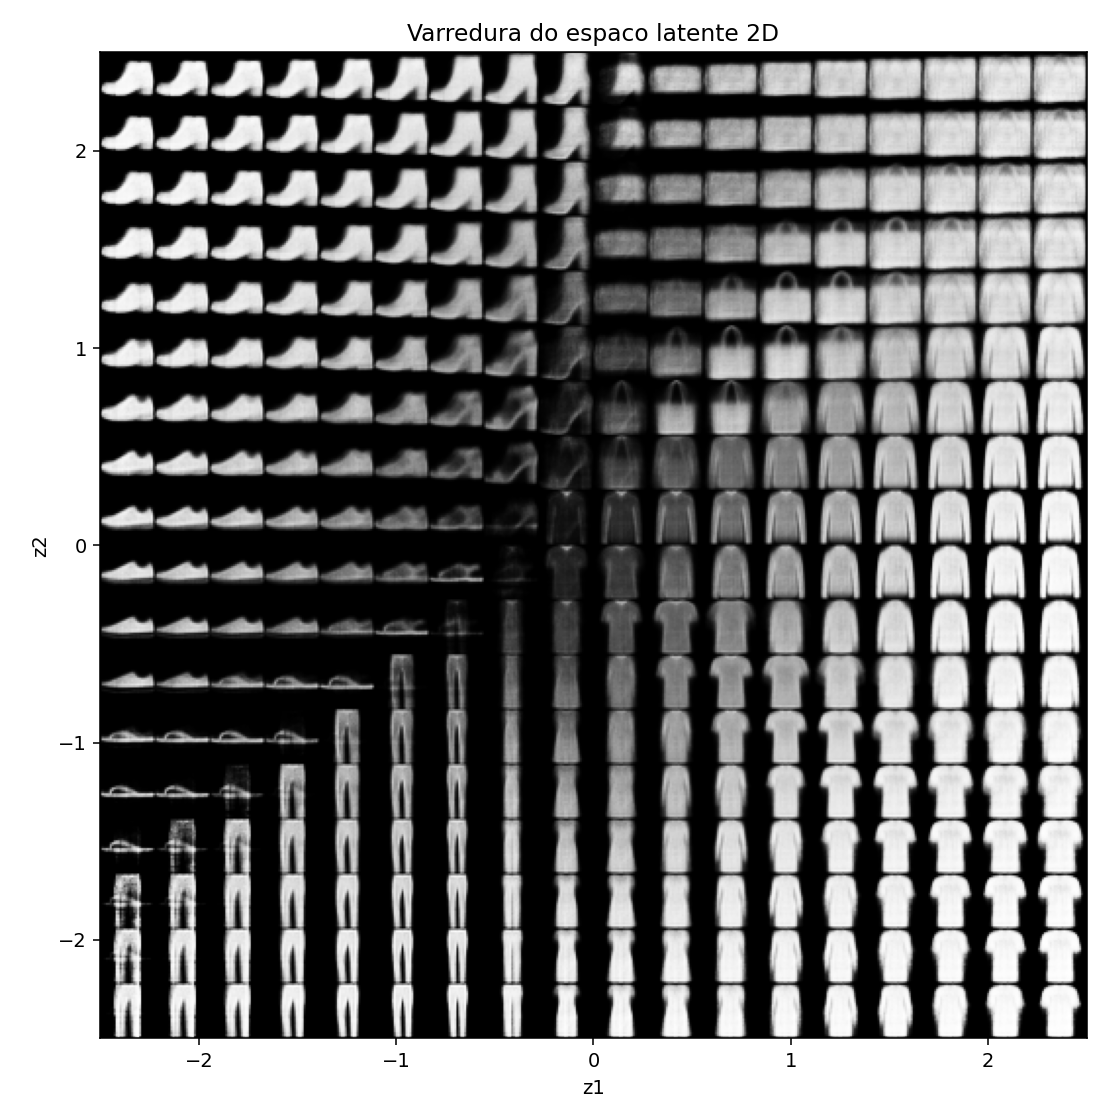
\includegraphics[width=0.62\textwidth]{../figures/latent2d_sweep.png}
\caption{Varredura do plano latente 2D: cada posição é decodificada em uma
imagem, revelando a organização contínua do espaço.}
\label{fig:sweep2d}
\end{figure}

\subsection{Espaço latente 8D projetado em 2D (PCA)}

\begin{figure}[H]
\centering
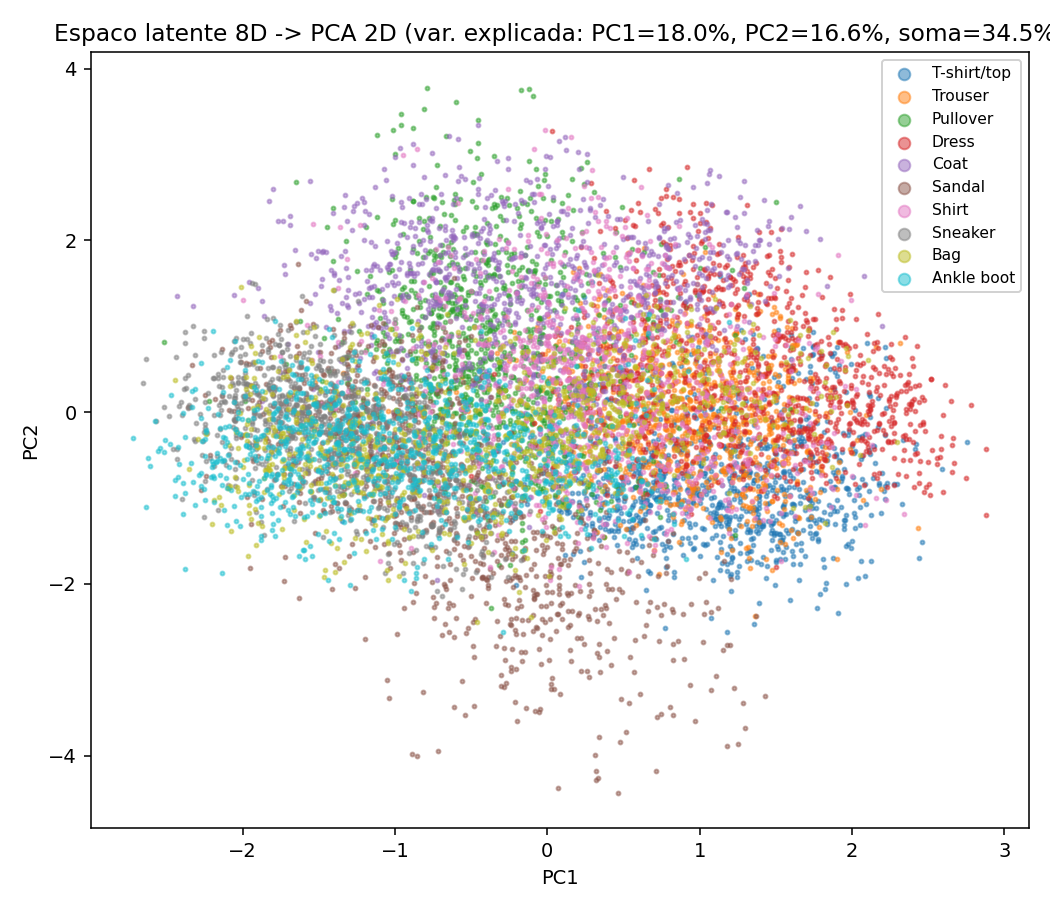
\includegraphics[width=0.74\textwidth]{../figures/latent8d_pca_scatter.png}
\caption{Projeção PCA (2 componentes) do espaço latente 8D, colorida pelos
rótulos.}
\label{fig:lat8d}
\end{figure}

A Figura~\ref{fig:lat8d} projeta o espaço 8D nos dois primeiros componentes
principais. Observa-se um gradiente por classe --- \textit{Dress} e
\textit{Trouser} à direita, calçados à esquerda, \textit{Coat} e
\textit{Pullover} na parte superior ---, mas a separação é visualmente menos
nítida que no caso 2D. Esse resultado deve ser interpretado com cautela: a
projeção retém apenas parte da informação, como detalhado a seguir.

A Figura~\ref{fig:var8d} mostra a variância explicada por componente. Os dois
primeiros componentes respondem por 18,0\% e 16,6\% da variância,
respectivamente, somando apenas \textbf{34,5\%}. Portanto, cerca de dois terços
da variância do espaço 8D residem nas seis dimensões descartadas pela projeção.
A aparência mais ``misturada'' da Figura~\ref{fig:lat8d} é, em boa parte, um
artefato da projeção, e não necessariamente ausência de estrutura no espaço 8D.

\begin{figure}[H]
\centering
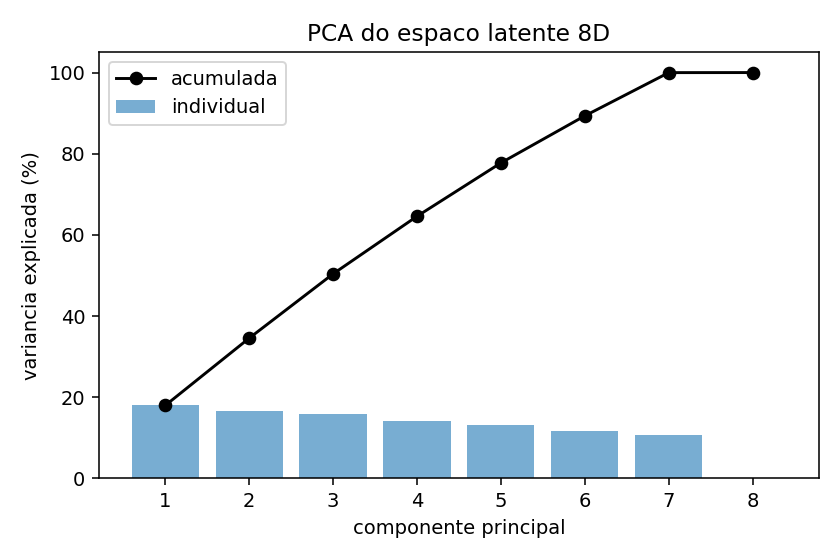
\includegraphics[width=0.6\textwidth]{../figures/latent8d_pca_variance.png}
\caption{Variância explicada (individual e acumulada) pelos componentes
principais do espaço latente 8D.}
\label{fig:var8d}
\end{figure}

\section{Respostas às Questões Propostas}

\paragraph{Há formação de \textit{clusters} no espaço latente?}
Sim. No espaço 2D, formam-se aglomerados visíveis, com destaque para
\textit{Trouser}, \textit{Bag} e o grupo de calçados, que ocupam regiões
contíguas e distintas. Os \textit{clusters} emergem de forma não supervisionada,
pois os rótulos não foram usados no treino.

\paragraph{Há separação dos rótulos no espaço latente?}
Parcialmente. A separação é boa entre grupos visualmente distintos (calçados,
calças, bolsas), mas as peças de parte superior do corpo (\textit{T-shirt},
\textit{Pullover}, \textit{Coat}, \textit{Dress}, \textit{Shirt}) permanecem
sobrepostas, refletindo sua semelhança de forma. O modelo 8D reconstrói melhor,
mas sua projeção 2D exibe separação visual menos nítida, principalmente por
limitação da própria projeção.

\paragraph{Quanto da variância a projeção ilustra?}
No caso 2D não há projeção: as duas dimensões são mostradas integralmente. No
caso 8D, a projeção PCA em dois componentes ilustra 34,5\% da variância total do
espaço latente (18,0\% no PC1 e 16,6\% no PC2). Assim, a visualização 8D
representa pouco mais de um terço da estrutura, o que ajuda a explicar por que os
rótulos parecem menos separados nessa figura.

\section{Conclusões}

Foram treinados dois VAEs para o Fashion-MNIST, com espaços latentes de 2 e 8
dimensões, selecionando-se a topologia pela loss de validação. O espaço 2D
privilegia a interpretabilidade: produz \textit{clusters} legíveis e um plano
latente contínuo, ao custo de reconstruções menos detalhadas. O espaço 8D
privilegia a fidelidade: reconstrói melhor as imagens, mas exige projeção para
ser visualizado, e dois componentes principais cobrem apenas 34,5\% da sua
variância. Em ambos os casos, observou-se organização dos rótulos de forma não
supervisionada, com separação clara entre grupos visualmente distintos e
sobreposição esperada entre peças de formato semelhante. O compromisso entre
compressão e fidelidade --- capturado pela decomposição do ELBO em reconstrução
e KL --- é, portanto, o fio condutor dos resultados.

\section*{Referências}

\begin{enumerate}
\item KINGMA, D. P.; WELLING, M. Auto-Encoding Variational Bayes. In:
\textit{International Conference on Learning Representations (ICLR)}, 2014.
\item XIAO, H.; RASUL, K.; VOLLGRAF, R. Fashion-MNIST: a Novel Image Dataset for
Benchmarking Machine Learning Algorithms. \textit{arXiv:1708.07747}, 2017.
\end{enumerate}

\end{document}
